\section{Performed optimization}\label{sec:yourmethod}
In this section we propose an optimized implementation of the quantization and Quantized Matrix-Matrix Multiplication (QMMM) functions introduced in \cref{sec:background} that uses four bits compression. We start by presenting the data structure that we use for our baseline implementation. We continue by analysing the bottlenecks of this implementation and by proposing a set of solutions to achieve a higher performance.

\mypar{Baseline implementation}
We presented the algorithm at the base of a straight forward implementation of a simple QNN using a $k$-bits compression scheme in \cref{sec:background}. Here we introduce the data structure necessary to a naive implementation in case $k=4$. Using a 4-bits compression scheme presents challenges due to the byte addressability of the computer memory and to the lack of a built-in 4-bits integer data type. As a consequence, we have to define our custom data structure. One way of operating on entities that require less than a byte for storage is to use structs in combination with bit fields. Nevertheless, byte addressability of the memory does not make it possible to load or store less than one byte at a time. Hence, using bit fields to define a custom data type that stores a single 4-bits integer is wasteful.  In the proposed solution we define the $uint4x4\_t$ data structure. This is a 2 bytes struct that exploits bit fields to store four integers of 4 bits each. Given a $n\times m$ weight matrix $\mathbf{A}$ of floats, its 4-bits quantized counterpart $\tilde{\mathcal{Q}}(\mathbf{A})$ is stored as an $\frac{n}{2}\times \frac{m}{2}$ matrix of $uint4x4\_t$. Because of this design choice, we assume both $n$ and $m$ to be even. In particular, the element $(i, j)$ of $\tilde{\mathcal{Q}}(\mathbf{A})$ contains the quantized representation of the elements of $\mathbf{A}$ at the following indices: $(2i, 2j),~(2i, 2j+1),~(2i+1, 2j),~(2i+1, 2j+1)$. The relation between the logical layout and the memory layout for the original matrix $\mathbf{A}$ and its quantized version that uses $uint4x4\_t$ data structure,   $\tilde{\mathcal{Q}}(\mathbf{A})$, can be seen in \cref{fig:uint4x4_t}. The difference between the memory layout of the $\mathbf{A}$ and $\tilde{\mathcal{Q}}(\mathbf{A})$ will play an important role in the vectorization of the code.
The reason why we pack four integers in one struct instead of two is that it allows us to define a data type that is more convenient for QMMM. Indeed the the definition of MMM applies as well for a matrix of $uint4x4\_t$, where the product and the sum of $uint4x4\_t$ elements are those of a 2x2 matrix. Then all the optimization techniques available for float MMM can be applied in $uint4x4\_t$ MMM.


\begin{figure}
\centering
  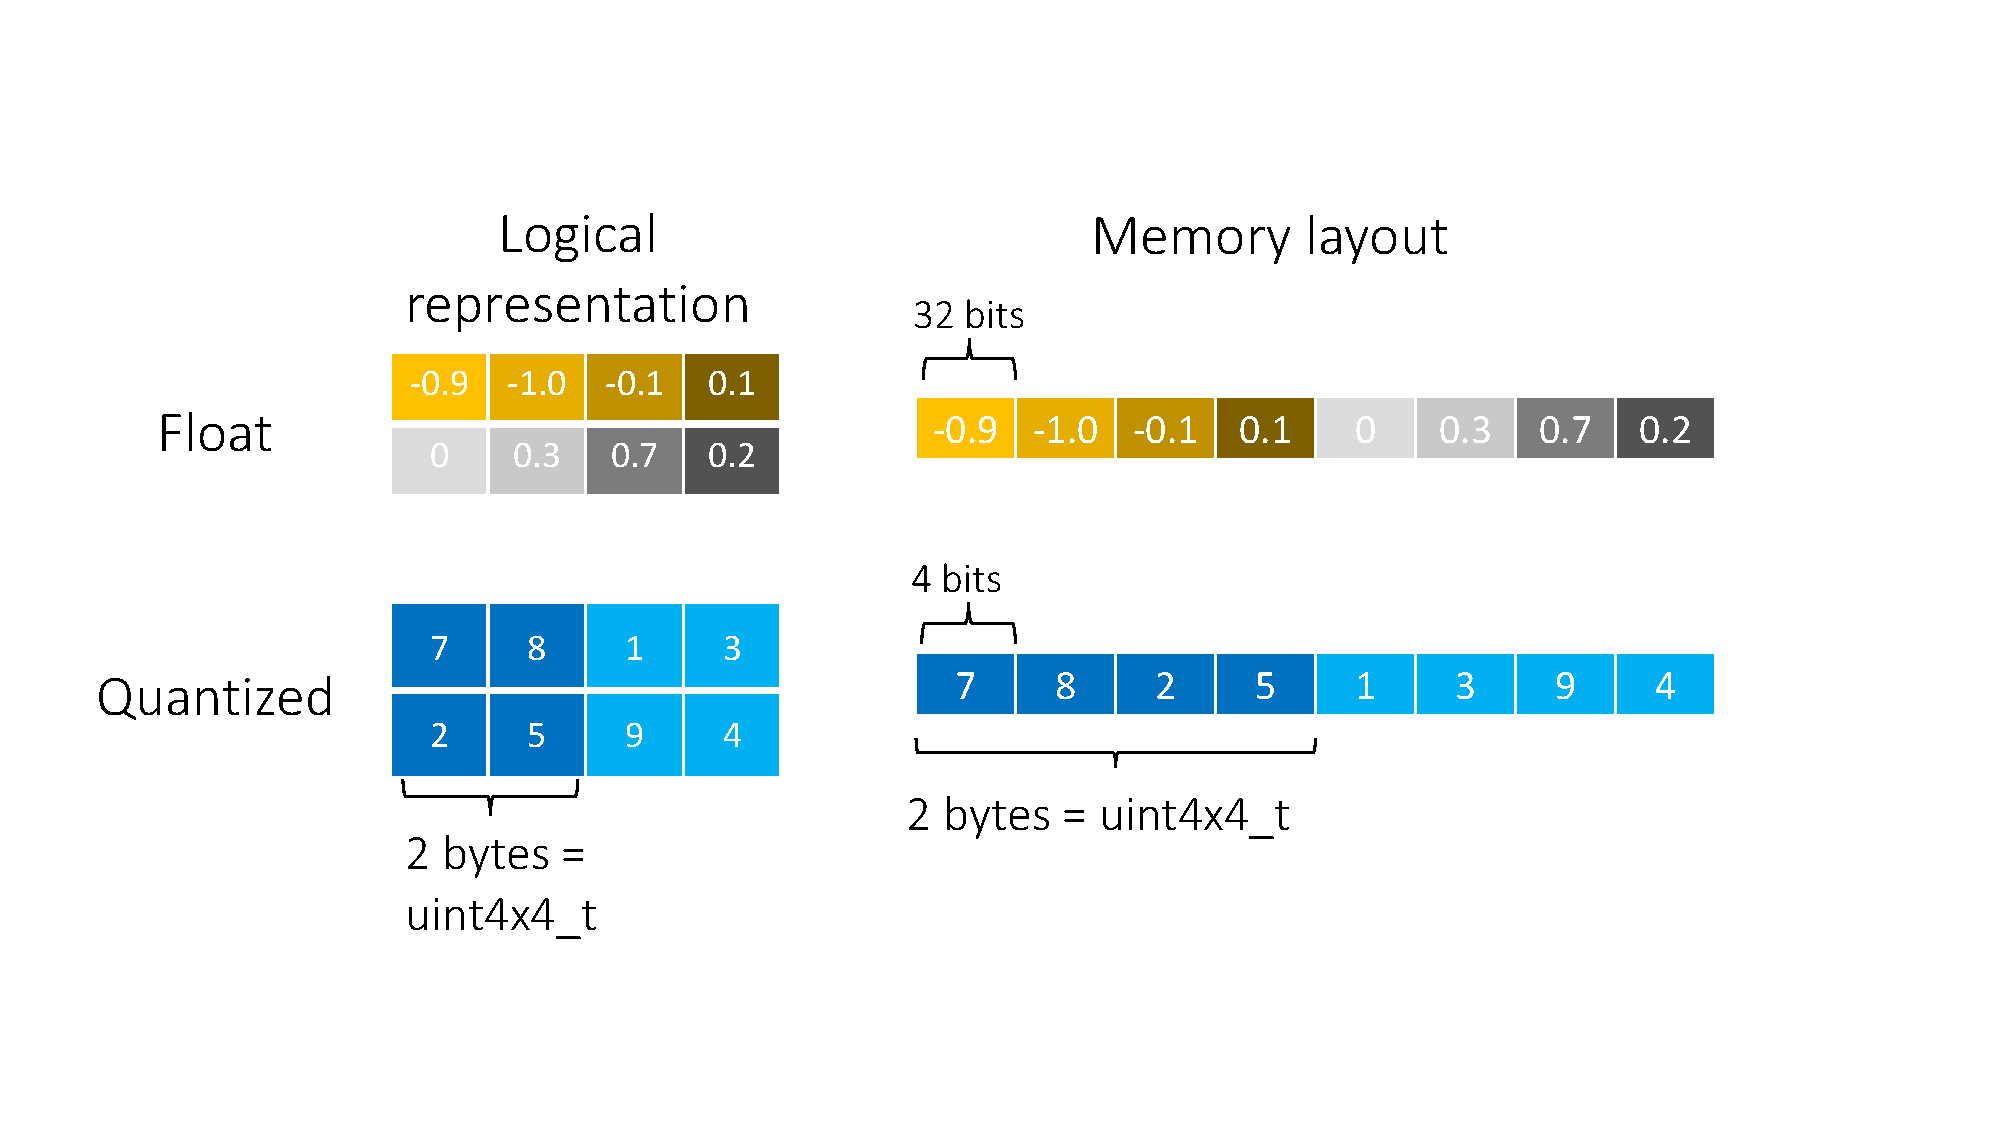
\includegraphics[scale=0.3]{figures/uint4x4_t.pdf}
  \caption{\label{fig:uint4x4_t}Logical and memory layouts of a weight matrix and its corresponding 4-bits quantized version stored as a matrix of $uint4x4\_t$. Cells that share the same color are stored in the same data structure. }
\end{figure}


\mypar{Operation count optimization}
The first optimization we present concerns the reduction of redundant computation. Using simple linear algebra, we can rewrite \cref{equation:qmmm} as:
\begin{align}\label{equation:qmmm_smart}
\begin{split}
\mathcal{Q}(\mathbf{L}) \mathcal{Q}(\mathbf{R}) = \Delta(\mathbf{L}) \Delta(\mathbf{R}) ( \tilde{\mathcal{Q}}(\mathbf{L}) \tilde{\mathcal{Q}}(\mathbf{R}) - z(\mathbf{L}) \mathbf{J} \tilde{\mathcal{Q}}(\mathbf{R}) + \\
- z(\mathbf{R}) \tilde{\mathcal{Q}}(\mathbf{L}) \mathbf{J} +  z(\mathbf{L}) z(\mathbf{R}) \mathbf{J} \mathbf{J} ).
\end{split}
\end{align}
This formulation of the QMMM makes it easy to see its redundant computation. The result of the product $\mathbf{J} \tilde{\mathcal{Q}}(\mathbf{R})$ contained in the second term inside the parenthesis is a matrix that has all rows equal to each other. In particular the $i^{th}$ term of any such row is the sum of the elements of the $i^{th}$ column of  $\tilde{\mathcal{Q}}(\mathbf{R})$. As a consequence, one can compute such row only once and save computation. In particular, this means we move ops from the inner most loop of the QMMM to the second  inner most loop. Thus, the count of such ops grows quadratically with the size of the weight matrix rather than cubically. A similar reasoning can be applied to the third and fourth term inside the parenthesis.

\mypar{Memory optimization}
Another important optimization of our implementation is related to the efficient use of the memory. To increase the temporal locality of the QMMM kernel, we exploit the well known blocking strategy, both for cache and for register. The parameter of the blocking are the cache-block size $N_b$ and the register-block size $n_b$, as outlined in \cref{fig:blocking} 

\begin{figure}
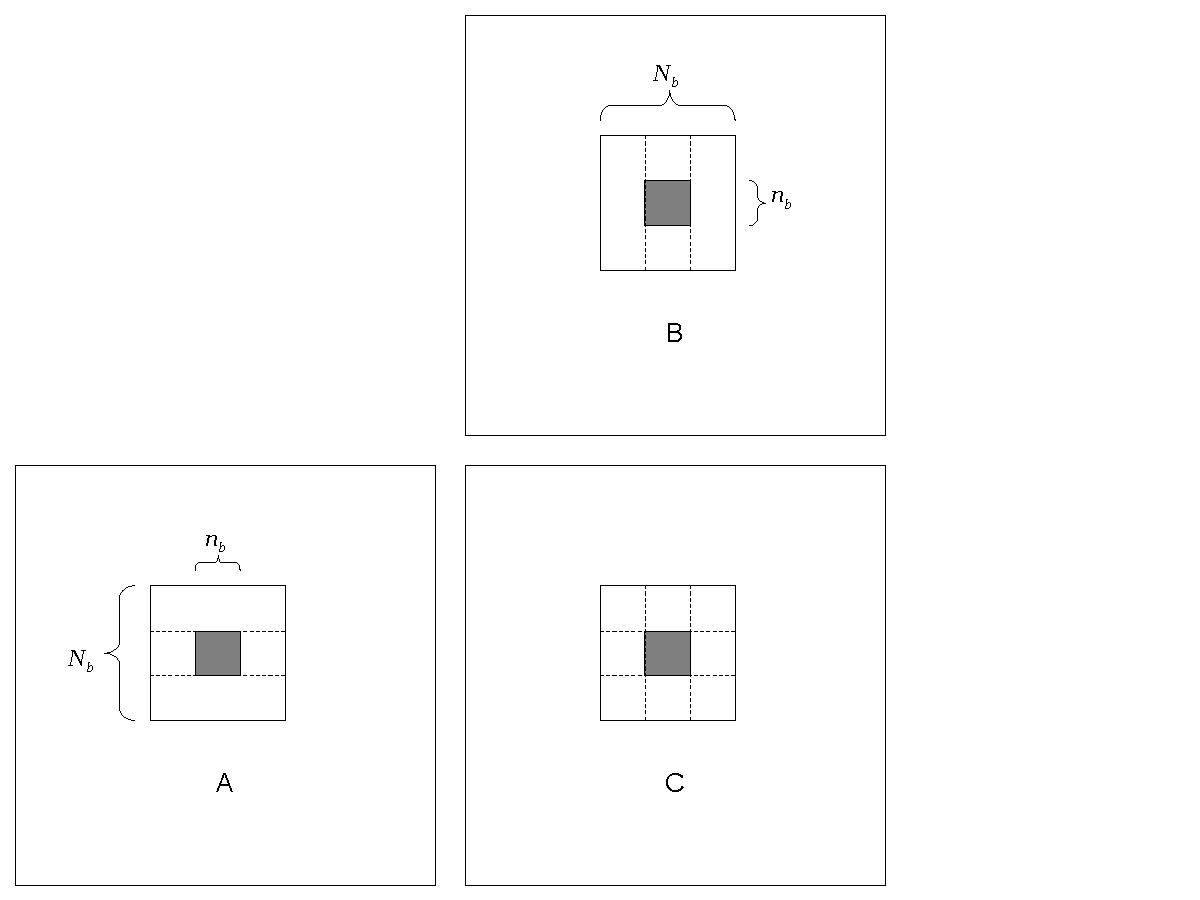
\includegraphics[scale=0.5]{figures/blocking}
\caption{Blocking parameters for the QMMM}
\label{fig:blocking}
\end{figure}


\mypar{Vectorization}
Finally, a critical aspect of our implementation concerns the vectorization of the code. The gain in performance that can be expected vary depending on what type of data a function operates on. For example, if we consider the functions needed to implement the quantization step, we can expect to observe a gain in performance up to $\times 8$ because an AVX register can operate on $8$ floats simultaneously. On the other hand, when we  consider the QMMM, in principle we can expect a gain in performance up to $\times 16$. This is because, in order to have the representation power that is necessary to compute correctly the dot products that appear in the term $ \tilde{\mathcal{Q}}(\mathbf{L}) \tilde{\mathcal{Q}}(\mathbf{R})$ of \cref{equation:qmmm_smart}, we use 16-bits integers as accumulators. As a consequence, our implementation of quantization and QMMM is divided into sub-functions that try to keep as separate as possible the integer computation from the float computation. Among them,  the most important are:

\begin{itemize}
\item \emph{round-sat}: computes the round and saturation operation used in line 5 of \cref{algorithm:quantize} and line 2 of \cref{algorithm:qmmm}.
\item \emph{quantize}: given a weight matrix $\mathbf{A}$ performs the operation necessary to compute  $\tilde{\mathcal{Q}}(\mathbf{A}) $ except for rounding and saturating (e.g. computing $mn$, $mx$, $\Delta(\mathbf{A})$).
\item \emph{qmmm\_kernel}: computes the  $uint4x4\_t$ MMM $ \tilde{\mathcal{Q}}(\mathbf{L}) \tilde{\mathcal{Q}}(\mathbf{R})$
\item \emph{trick}: computes the sum over columns and rows of $\tilde{\mathcal{Q}}(\mathbf{R})$ and $\tilde{\mathcal{Q}}(\mathbf{L})$ respectively. As explained before, this is needed to reduce the overall ops count of QMMM. 
\item \emph{add\_trick}: adds the appropriate element of the row and the columns computed by the \emph{trick} function to the result of the dot product computed by \emph{qmmm\_kernel}.
\end{itemize}
\Cref{tab:cost} summarizes the cost in FLOPS or IOPS of each of the functions above.

\begin{table}
\centering
\begin{tabular}{ c|c } 
 
 Function & Ops count (int or float) \\
 \hline 
 \emph{round-sat} & $5N^2$ FLOPS \\
\emph{quantize} & $7N^2$ FLOPS \\
\emph{qmmm\_kernel} & $2N^3$ IOPS \\
\emph{trick} & $2N^2 + 2N$ IOPS \\
\emph{add\_trick} & $3N^3$ IOPS \\
 \end{tabular}
  \caption{Cost analysis}
\label{tab:cost} 
\end{table}

Among the numerous advantages in terms of performance that come from using 4-bits compression, there are also drawbacks due to the memory layout of the $uint4x4\_t$ data structure shown in \cref{fig:uint4x4_t}. For example, listing \ref{list:load_row} shows the overhead in terms of masking, shifting and blending that is required to load two rows of the quantized weight matrix.

\lstinputlisting[language=C++, caption={Load of two $uint4x4\_t$ rows.}, label={list:load_row}]{figures/load.cpp}